%*****************************************
\chapter{Grundlagen}\label{ch:grundlagen}
%*****************************************
Grundlagen die untersucht werden Intrusion Detection System (IDS) sowie die spezielle Form der RNNs die LSTM-NN
Erster Abschnitt beschreibt verschiedene IDS Ansätze
Hierbei auch auf die verwendete Anomalieerkennung
Dann soll der verwendete Datensatz beschrieben werden
Abschließend LSTM

    \section{Intrusion Detection System}
        Erkennen von Angriffen auf Computersysteme
        \subsection{Ansätze}
            \begin{itemize}
                \item Signaturbasiert
                    \begin{itemize}
                        \item Whitelist
                        \item Blacklist
                            \subitem aufzählen aller Angriffe
                    \end{itemize}
                \item Anomaliebasiert
                    \subitem Definiere was normal ist
                    \subitem Analogie menschliches Immunsystem
                    $\rightarrow$ Auch NN Analogie zur Natur <++> 
                    Host Based, Network traffic, logging
            \end{itemize}
        \subsection{Host Based Intrusion Detection}
        Überwacht system intern, zum beispiel Kernel --> System calls verbinung Kernel Programme
    \section{Anomalieerkennung}
        Anomalien sind Muster die nicht einem wohldefinierten Normalverhalten entsprechen
        Ziel der Anomalieerkennung ist es Muster in Daten wieder zu erkennen
        Normalverhalten muss in Daten wiedergespiegelt werden
        überwacht --> gelabelt normalverhalten und anormales
        -> problem overfitting von anormalen verhalten
        unüberwacht
        semi überwacht --> nur normalverhalten, liegt hier vor aber gelabelt testdaten
        benötigt Schwellwert --->  siehe Kapitel algorithm
        wird dieser überschritten 
        Es gibt verschiedene Arten von anomalien
        \subsection{System Calls}
        \subsubsection{System Call Arguments}
        \paragraph{String Length}
        \paragraph{String Character Distribution}
        \paragraph{Structural Inference}
        \paragraph{Token Finder}
        
    \section{Künstliche neuronale Netze}
        
        Das Nutzen von bestehenden und in der Natur vorkommenden Strukturen und Abfolgen kommt in verschiedenen Bereichen zum Einsatz.
        Sehr bekannt dabei sind zum Beispiel ---
        Ein in den letzten Jahren immmer weiter verbreiteter Ansatz ist in der Informatik die Verwendung von künstlichen neuronalen Netzen, welcher sich die Struktur von Gehirnen zu eigen macht.
        Man verspricht sich mit dem Einsatz von künstlichen neuronale Netze, welche eine varietät von verschiedenen Architekturen beinhalten, diverse Optimierungsprobleme zu lösen.
        In dieser Arbeit wird der Einsatz von neuronalen Netzen zur \textit{Time Series Prediction} (zu dt. Vorhersagen von Zeitreihen) untersucht.
        Für die \textit{Time Series Prediction} sind verschieden Architekturen von neuronalen Netzen weit verbreitet \cite{BENIDIS2020}.
        Zu aktuellen Beispielen zählen dabei auch Vorhersagen die im Zusammenhang mit der Verbreitung des COVID-19 Virus stehen \cite{COVID1} \cite{COVID2} \cite{COVID3}.

        % überarbeiten
        unterteilung verschiedener Netze und einordnung von rnns und lstmnn
        
        %Neuronale Netze bestehen aus verschiedenen Ebenen von Knoten (auch Neuronen genannt), die miteinander verbunden sind.
        %Die Neuronen erhalten Eingangssignale und falls diese eine bestimmte Bedingung erfüllen (z.B. Schwellwertüberschreitung) wird das Ausgangssignal des Neurons verändert.
        %Wird die Bedingung nicht erfüllt, sendet das Neuron ein Signal, welches die nachfolgenden Neuronen nicht beeinflusst. Der schematische Aufbau wird in Abbildung \ref{fig:Neuron} gezeigt.
%
            %\begin{figure}[ht]
                %\centering
                %\includegraphics[width=0.4\textwidth]{images/Neron}
                %\caption{Aufbau eines Neurons}
                %\label{fig:Neuron}
            %\end{figure}
            %\begin{figure}[ht]
                %\centering
                %\includegraphics[width=0.5\textwidth]{images/NeuralNet}
                %\caption{Schematische Darstellung eines neuronalen Netzes}
                %\label{fig:NeuralNet}
            %\end{figure}
        %
            %\begin{figure}[ht]
                %\centering
                %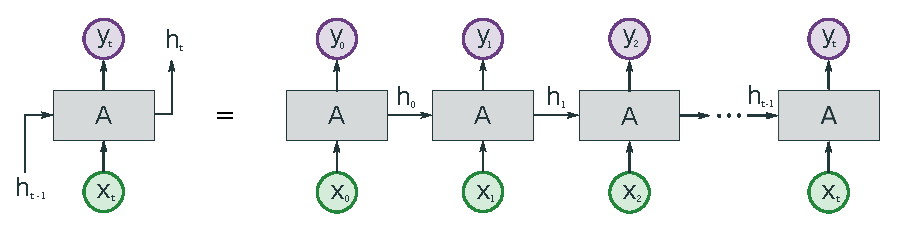
\includegraphics[width=0.8\textwidth]{images/Illustrationen/RNN}
                %\caption{\glqq Ausgerollte\grqq \ Darstellung eines RNN Neurons (inspiriert von \cite{OLAH2015})}
                %\label{fig:RNN}
            %\end{figure}
            %
        %Da ein einzelnes Neuron noch keine komplexen Aufgaben lösen kann, ist der Aufbau in Netzen entscheidend.
        %Die Neuronen sind in sogenannten \textit{Layers} (z dt. Ebenen) angeordnet (siehe Abbildung \ref{fig:NeuralNet}).
        %Es gibt eine \textit{Input-Layer}, quasi beliebig viele \textit{Hidden-Layers} und eine \textit{Output-Layer}.
        %Die einzelnen Knoten sind jeweils mit der nachfolgenden Layer verbunden.
        %Ist der Ausgang eines Knotens auf einer Layer mit einer vorherigen oder derselben Layer verbunden, spricht man von einem \textit{Feedback} oder \textit{Recurrent Neural Network} (RNN) (siehe Abbildung \ref{fig:RNN}), sonst von einem \textit{Feedforward Neural Network} (FNN). 
        %Mit Knoten, die eine extra Verbindung zu sich selbst haben, können frühere Eingaben Einfluss auf die Behandlung der nächsten Eingabe haben.
        %Der einzelne Knoten merkt sich seine Ausgabe, welche im nächsten Zeitschritt als weiteres Eingabesignal dient.
        %Dadurch wird es ermöglicht auch zeitlich abhängige Sequenzen zu erlernen, da die Behandlung eben auch vorherige Geschehnisse mit einbezieht.
        %Wird ein FNN zum Beispiel lediglich auf die Eingabe (A,B,A,B,A,B,A,\dots) trainiert, besteht eine 50\% Chance, dass die nächste Ausgabe ein B ist, sofern die Trainingsdaten korrekt im FNN abgebildet sind.
        %Ein Hauptgrund dafür ist, dass die voherige Eingabe nicht bekannt ist.
        %Ist bekannt, dass die letzte Ausgabe ein B war, können wir davon ausgehen, dass eigentlich ein A folgen sollte.
        %Durch die Feedback Struktur der RNNs liefert also einen ersten Ansatz, um zeitlich abhängige Muster besser zu erkennen.

    \subsection{Long Short-Term Memory Recurrent Neural Network}
    
    
    	\begin{figure}[ht]
    		\centering
    		\includegraphics[width=0.8\textwidth]{images/Illustrationen/LSTM}
    		\caption{Schematische Darstellung eines Knotens in einem LSTM NN, mit Input, Output und Forget Gate (inspiriert von \cite{OLAH2015}).}
    		\label{fig:LSTM}
    	\end{figure}
   	
        \textit{Long Short-Term Memory} (LSTM) ist eine Erweiterung der RNNs.
        Hauptziel der LSTMs ist es, das Lernen der zeitlich abhängigen Muster zu verbessern.
        Auch RNNs haben dieses Ziel, doch mit diesen Netzwerken kann schon ein Abstand von 10 diskreten Zeitschritten zwischen den abhängigen Ereignissen nicht überbrückt werden \cite{HOCHREITER1991}. 
        So kann ein RNN sofern es korrekt trainiert wurde mit hoher Wahrscheinlichkeit im Satz \glqq Die Wolken am \textit{Himmel}\grqq \ das Wort \textit{Himmel} vorhersagen, doch bei der Satzfolge \glqq Die Person kommt aus Frankreich. ... . Die Person spricht \textit{französisch}.\grqq \ wird es Schwierigkeiten haben.
        Ein weitere Problemstellung mit RNNs ist das stabile trainieren.
        Dabei kommt es häufig vor, dass durch die Back Propagation die berechneten Gradienten entweder verschwindend klein, oder sehr groß werden.
        Gerade bei Abhängigkeiten über einen größeren zeitlichen Abstand tendieren die Fehlersignale, die durch die Back Propagation durch das Netz gegeben werden, zu geringe Gewichtsänderungen auszulösen \cite{HOCHREITER1998}.
        Die LSTM Zelle ermöglichen durch verbesserte Fehlerkorrektur stabilere Lernergebnisse sowie auch das Lernen von Mustern mit noch größeren zeitlichen Abstände.
        Umgesetzt wird diese Anforderung, indem an jedem Knoten eine \textit{Memory Cell} (Gedächtniszelle) angebracht wird \ref{fig:LSTM}.
        Sie ist mit sich selbst verbunden und gibt den Zellstatus an.
        Mit Hilfe dieser Information soll eine Abhängigkeit auch über einen längeren Zeitraum gefunden werden.
        Der Zellstatus $C_{t-1}$ zum Zeitpunkt $t-1$ hat dann im nächsten Zeitschritt $t$ einen Einfluss auf den Zellstatus $C_{t}$ und somit auch auf die Ausgabe $y_t$.
        Die Weitergabe des Status wird in Abbildung \ref{fig:LSTM_Status} dargestellt.

            \begin{figure}[ht]
                \centering
                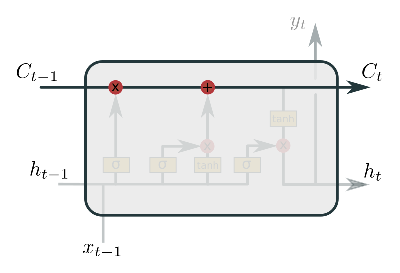
\includegraphics[width=0.5\textwidth]{images/Illustrationen/LSTM_MC}
                \caption{Weitergabe des Zellstatus innerhalb eines Knotens (inspiriert von \cite{OLAH2015}).}
                \label{fig:LSTM_Status}
            \end{figure}
            
        Einfluss auf den Zellstatus haben zwei verschiedene \textit{Gates} (zu dt. Gatter/Tore).
        Im ersten Schritt wird entschieden, welche Information aus dem vorherigen Zeitschritt keinen Einfluss mehr auf den Zellstatus haben sollen.
        Dies wird mit dem \textit{Forget Gate} umgesetzt und ist in Abbildung \ref{fig:LSTM_Forget} zu sehen.
        Informationen aus dem Speicher, die keinen Einfluss mehr haben sollen, können so entfernt werden.
        In dem Sprachbeispiel könnte das Genus (\textit{grammatikalisches Geschlecht}) gespeichert werden, um so eine grammatikalisch korrekte Vorhersage zu machen.
        Kommt nun allerdings ein neues Pronomen, sollte das bisher gespeicherte Genus keinen Einfluss mehr haben.
            \begin{figure}[ht]
                \centering
                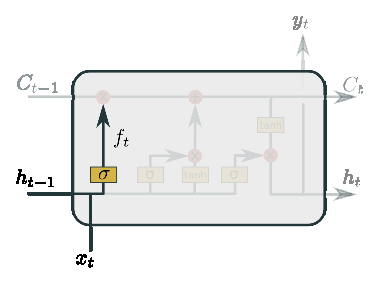
\includegraphics[width=0.5\textwidth]{images/Illustrationen/LSTM_FG}
                \caption{Einfluss des Forget Gates auf den Zellstatus (inspiriert von \cite{OLAH2015}).}
                \label{fig:LSTM_Forget}
            \end{figure}
            
        Das \textit{Input Gate} soll im nächsten Schritt angeben, welche neuen Informationen in den Zellstatus $C_t$ aufgenommen werden.
        Dies erfolgt in zwei Schritten, zunächst wird mit $i_t$ ermittelt, welche Information geupdated werden soll.
        Im Vektor $\tilde{C}$ ist der eigentliche Werte (wie z.B. das Genus) enthalten, welcher den zuvor vergessenen Wert ersetzen soll (vgl. Abbildung \ref{fig:LSTM_Input}) . 
            \begin{figure}[ht]
                \centering
                \includegraphics[width=0.5\textwidth]{images/Illustrationen/LSTM_IG2}
                \caption{Einfluss des Input Gates auf den Zellstatus (inspiriert von \cite{OLAH2015}).}
                \label{fig:LSTM_Input}
            \end{figure}
        
        Wie der Zellstatus $C_t$ nun die Ausgabe beeinflusst, wird über das \textit{Output Gate} geregelt (siehe Abbildung \ref{fig:LSTM_Output}).
        Dies soll in unserem Sprachbeispiel entscheiden, ob die Information des Genus für die Vorhersage des nächsten Wortes eine Rolle spielt. \cite{GERS2000} \cite{OLAH2015}
            \begin{figure}[ht]
                \centering
                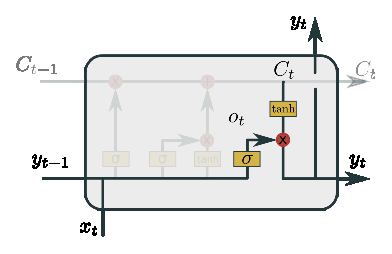
\includegraphics[width=0.5\textwidth]{images/Illustrationen/LSTM_OG}
                \caption{Das Output Gate regelt den Einfluss des Zellstatus auf die Ausgabe des Neurons (inspiriert von \cite{OLAH2015}).}
                \label{fig:LSTM_Output}
            \end{figure}
        
        Die verschiedenen Gates können so als ein weiteres kleines NN in jedem Knoten der LSTM Netze betrachtet werden, welche einen zeitlichen Zusammenhang besser erkennen sollen.
    
        \subsection{Word2Vec}
